\documentclass[a4paper]{article}

\def\nterm {Spring}
\def\nyear {2020}
\def\nlecturer {Dan Perelstein}
\def\ncourse {Sound Systems Design and Engineering}

\RequirePackage{etex}
\makeatletter
\ifx \nauthor\undefined
  \def\nauthor{Daniel Moore}
\else
\fi

\author{Based on lectures by \nlecturer \\\small Notes taken by \nauthor}
\date{\nterm\ \nyear}

\usepackage{alltt}
\usepackage{amsfonts}
\usepackage{amsmath}
\usepackage{amssymb}
\usepackage{amsthm}
\usepackage{booktabs}
\usepackage[makeroom]{cancel}
\usepackage{caption}
\usepackage{enumitem}
\usepackage{fancyhdr}
\usepackage{graphicx}
\usepackage{mathdots}
\usepackage{mathtools}
\usepackage{microtype}
\usepackage{multirow}
\usepackage{pdflscape}
\usepackage{pgfplots}
\usepackage{siunitx}
\usepackage{textcomp}
\usepackage{slashed}
\usepackage{tabularx}
\usepackage{tikz}
\usepackage{tikz-3dplot}
\usepackage{tkz-euclide}
\usepackage{titlesec}
\usepackage[normalem]{ulem}
\usepackage[all]{xy}
\usepackage{imakeidx}

\makeindex[intoc, title=Index]
\indexsetup{othercode={\lhead{\emph{Index}}}}
%\setcounter{secnumdepth}{4}

\titleformat{\paragraph}
{\normalfont\normalsize\bfseries}{\theparagraph}{1em}{}
\titlespacing*{\paragraph}
{0pt}{3.25ex plus 1ex minus .2ex}{1.5ex plus .2ex}

\ifx \nextra \undefined
  \usepackage[pdftex,
    hidelinks,
    pdfauthor={Daniel Moore},
    pdfsubject={\ncourse},
    pdftitle={\ncourse},
  pdfkeywords={\nterm\ \nyear\ \ncourse}]{hyperref}
  \title{\ncourse}
\else
  \usepackage[pdftex,
    hidelinks,
    pdfauthor={Daniel Moore},
    pdfsubject={\ncourse\ (\nextra)},
    pdftitle={\ncourse\ (\nextra)},
  pdfkeywords={\nterm\ \nyear\ \ncourse\ \nextra}]{hyperref}

  \title{\ncourse \\ {\Large \nextra}}
  \renewcommand\printindex{}
\fi

\pgfplotsset{compat=1.12}

\pagestyle{fancyplain}
\ifx \ncoursehead \undefined
\def\ncoursehead{\ncourse}
\fi

\lhead{\emph{\nouppercase{\leftmark}}}
\ifx \nextra \undefined
  \rhead{
    \ifnum\thepage=1
    \else
      \ncoursehead
    \fi}
\else
  \rhead{
    \ifnum\thepage=1
    \else
      \ncoursehead \ (\nextra)
    \fi}
\fi
\usetikzlibrary{arrows.meta}
\usetikzlibrary{decorations.markings}
\usetikzlibrary{decorations.pathmorphing}
\usetikzlibrary{positioning}
\usetikzlibrary{fadings}
\usetikzlibrary{intersections}
\usetikzlibrary{cd}

\newcommand*{\Cdot}{{\raisebox{-0.25ex}{\scalebox{1.5}{$\cdot$}}}}
\newcommand {\pd}[2][ ]{
  \ifx #1 { }
    \frac{\partial}{\partial #2}
  \else
    \frac{\partial^{#1}}{\partial #2^{#1}}
  \fi
}
\newcommand{\pder}[2]{
    \frac{\partial #1}{\partial #2}
}
\newcommand{\dd}[1]{
	\frac{\d}{\d #1}
}
\newcommand{\der}[2]{
	\frac{\d #1}{\d #2}
}
\newcommand{\mbeq}{\overset{!}{=}}
\newcommand{\vhat}[1]{\vec{\hat{#1}}}
\newcommand{\x}{\vhat{x}}
\newcommand{\y}{\vhat{y}}
\newcommand{\z}{\vhat{z}}
\newcommand{\del}{\vec{\nabla}}
\ifx \nhtml \undefined
\else
  \renewcommand\printindex{}
  \DisableLigatures[f]{family = *}
  \let\Contentsline\contentsline
  \renewcommand\contentsline[3]{\Contentsline{#1}{#2}{}}
  \renewcommand{\@dotsep}{10000}
  \newlength\currentparindent
  \setlength\currentparindent\parindent

  \newcommand\@minipagerestore{\setlength{\parindent}{\currentparindent}}
  \usepackage[active,tightpage,pdftex]{preview}
  \renewcommand{\PreviewBorder}{0.1cm}

  \newenvironment{stretchpage}%
  {\begin{preview}\begin{minipage}{\hsize}}%
    {\end{minipage}\end{preview}}
  \AtBeginDocument{\begin{stretchpage}}
  \AtEndDocument{\end{stretchpage}}

  \newcommand{\@@newpage}{\end{stretchpage}\begin{stretchpage}}

  \let\@real@section\section
  \renewcommand{\section}{\@@newpage\@real@section}
  \let\@real@subsection\subsection
  \renewcommand{\subsection}{\@ifstar{\@real@subsection*}{\@@newpage\@real@subsection}}
\fi
\ifx \ntrim \undefined
\else
  \usepackage{geometry}
  \geometry{
    papersize={379pt, 699pt},
    textwidth=345pt,
    textheight=596pt,
    left=17pt,
    top=54pt,
    right=17pt
  }
\fi

\ifx \nisofficial \undefined
\let\@real@maketitle\maketitle
\renewcommand{\maketitle}{\@real@maketitle\begin{center}\begin{minipage}[c]{0.9\textwidth}\centering\footnotesize These notes are not endorsed by the lecturers, and I have modified them (often significantly) after lectures. They are nowhere near accurate representations of what was actually lectured, and in particular, all errors are almost surely mine.\end{minipage}\end{center}}
\else
\fi

% Theorems
\theoremstyle{definition}
\newtheorem*{aim}{Aim}
\newtheorem*{axiom}{Axiom}
\newtheorem*{claim}{Claim}
\newtheorem*{cor}{Corollary}
\newtheorem*{conjecture}{Conjecture}
\newtheorem*{defi}{Definition}
\newtheorem*{eg}{Example}
\newtheorem*{ex}{Exercise}
\newtheorem*{fact}{Fact}
\newtheorem*{law}{Law}
\newtheorem*{lemma}{Lemma}
\newtheorem*{notation}{Notation}
\newtheorem*{prop}{Proposition}
\newtheorem*{question}{Question}
\newtheorem*{problem}{Problem}
\newtheorem*{rrule}{Rule}
\newtheorem*{thm}{Theorem}
\newtheorem*{assumption}{Assumption}

\newtheorem*{remark}{Remark}
\newtheorem*{warning}{Warning}
\newtheorem*{exercise}{Exercise}

\newtheorem{nthm}{Theorem}[section]
\newtheorem{nlemma}[nthm]{Lemma}
\newtheorem{nprop}[nthm]{Proposition}
\newtheorem{ncor}[nthm]{Corollary}


\renewcommand{\labelitemi}{--}
\renewcommand{\labelitemii}{$\circ$}
\renewcommand{\labelenumi}{(\roman{*})}

\let\stdsection\section
\renewcommand\section{\newpage\stdsection}

% Strike through
\def\st{\bgroup \ULdepth=-.55ex \ULset}


%%%%%%%%%%%%%%%%%%%%%%%%%
%%%%% Maths Symbols %%%%%
%%%%%%%%%%%%%%%%%%%%%%%%%

% Matrix groups
\newcommand{\GL}{\mathrm{GL}}
\newcommand{\Or}{\mathrm{O}}
\newcommand{\PGL}{\mathrm{PGL}}
\newcommand{\PSL}{\mathrm{PSL}}
\newcommand{\PSO}{\mathrm{PSO}}
\newcommand{\PSU}{\mathrm{PSU}}
\newcommand{\SL}{\mathrm{SL}}
\newcommand{\SO}{\mathrm{SO}}
\newcommand{\Spin}{\mathrm{Spin}}
\newcommand{\Sp}{\mathrm{Sp}}
\newcommand{\SU}{\mathrm{SU}}
\newcommand{\U}{\mathrm{U}}
\newcommand{\Mat}{\mathrm{Mat}}

% Matrix algebras
\newcommand{\gl}{\mathfrak{gl}}
\newcommand{\ort}{\mathfrak{o}}
\newcommand{\so}{\mathfrak{so}}
\newcommand{\su}{\mathfrak{su}}
\newcommand{\uu}{\mathfrak{u}}
\renewcommand{\sl}{\mathfrak{sl}}

% Special sets
\newcommand{\C}{\mathbb{C}}
\newcommand{\CP}{\mathbb{CP}}
\newcommand{\GG}{\mathbb{G}}
\newcommand{\N}{\mathbb{N}}
\newcommand{\Q}{\mathbb{Q}}
\newcommand{\R}{\mathbb{R}}
\newcommand{\RP}{\mathbb{RP}}
\newcommand{\T}{\mathbb{T}}
\newcommand{\Z}{\mathbb{Z}}
\renewcommand{\H}{\mathbb{H}}

% Brackets
\newcommand{\abs}[1]{\left\lvert #1\right\rvert}
\newcommand{\bket}[1]{\left\lvert #1\right\rangle}
\newcommand{\brak}[1]{\left\langle #1 \right\rvert}
\newcommand{\braket}[2]{\left\langle #1\middle\vert #2 \right\rangle}
\newcommand{\bra}{\langle}
\newcommand{\ket}{\rangle}
\newcommand{\norm}[1]{\left\lVert #1\right\rVert}
\newcommand{\normalorder}[1]{\mathop{:}\nolimits\!#1\!\mathop{:}\nolimits}
\newcommand{\tv}[1]{|#1|}
\renewcommand{\vec}[1]{\boldsymbol{\mathbf{#1}}}

% not-math
\newcommand{\bolds}[1]{{\bfseries #1}}
\newcommand{\cat}[1]{\mathsf{#1}}
\newcommand{\ph}{\,\cdot\,}
\newcommand{\term}[1]{\emph{#1}\index{#1}}
\newcommand{\phantomeq}{\hphantom{{}={}}}
% Probability
\DeclareMathOperator{\Bernoulli}{Bernoulli}
\DeclareMathOperator{\betaD}{beta}
\DeclareMathOperator{\bias}{bias}
\DeclareMathOperator{\binomial}{binomial}
\DeclareMathOperator{\corr}{corr}
\DeclareMathOperator{\cov}{cov}
\DeclareMathOperator{\gammaD}{gamma}
\DeclareMathOperator{\mse}{mse}
\DeclareMathOperator{\multinomial}{multinomial}
\DeclareMathOperator{\Poisson}{Poisson}
\DeclareMathOperator{\var}{var}
\newcommand{\E}{\mathbb{E}}
\newcommand{\Prob}{\mathbb{P}}

% Algebra
\DeclareMathOperator{\adj}{adj}
\DeclareMathOperator{\Ann}{Ann}
\DeclareMathOperator{\Aut}{Aut}
\DeclareMathOperator{\Char}{char}
\DeclareMathOperator{\disc}{disc}
\DeclareMathOperator{\dom}{dom}
\DeclareMathOperator{\fix}{fix}
\DeclareMathOperator{\Hom}{Hom}
\DeclareMathOperator{\id}{id}
\DeclareMathOperator{\image}{image}
\DeclareMathOperator{\im}{im}
\DeclareMathOperator{\re}{re}
\DeclareMathOperator{\tr}{tr}
\DeclareMathOperator{\Tr}{Tr}
\newcommand{\Bilin}{\mathrm{Bilin}}
\newcommand{\Frob}{\mathrm{Frob}}

% Others
\newcommand\ad{\mathrm{ad}}
\newcommand\Art{\mathrm{Art}}
\newcommand{\B}{\mathcal{B}}
\newcommand{\cU}{\mathcal{U}}
\newcommand{\Der}{\mathrm{Der}}
\newcommand{\D}{\mathrm{D}}
\newcommand{\dR}{\mathrm{dR}}
\newcommand{\exterior}{\mathchoice{{\textstyle\bigwedge}}{{\bigwedge}}{{\textstyle\wedge}}{{\scriptstyle\wedge}}}
\newcommand{\F}{\mathbb{F}}
\newcommand{\G}{\mathcal{G}}
\newcommand{\Gr}{\mathrm{Gr}}
\newcommand{\haut}{\mathrm{ht}}
\newcommand{\Hol}{\mathrm{Hol}}
\newcommand{\hol}{\mathfrak{hol}}
\newcommand{\I}{\mathbb{I}}
\newcommand{\Id}{\mathrm{Id}}
\newcommand{\Lp}{\mathcal{L}}
\newcommand{\lie}[1]{\mathfrak{#1}}
\newcommand{\op}{\mathrm{op}}
\newcommand{\Oc}{\mathcal{O}}
\newcommand{\pr}{\mathrm{pr}}
\newcommand{\Ps}{\mathcal{P}}
\newcommand{\pt}{\mathrm{pt}}
\newcommand{\qeq}{\mathrel{``{=}"}}
\newcommand{\Rs}{\mathcal{R}}
\newcommand{\Vect}{\mathrm{Vect}}
\newcommand{\wsto}{\stackrel{\mathrm{w}^*}{\to}}
\newcommand{\wt}{\mathrm{wt}}
\newcommand{\wto}{\stackrel{\mathrm{w}}{\to}}
\renewcommand{\d}{\mathrm{d}}
\renewcommand{\P}{\mathbb{P}}
%\renewcommand{\F}{\mathcal{F}}


\let\Im\relax
\let\Re\relax

\DeclareMathOperator{\area}{area}
\DeclareMathOperator{\card}{card}
\DeclareMathOperator{\ccl}{ccl}
\DeclareMathOperator{\ch}{ch}
\DeclareMathOperator{\cl}{cl}
\DeclareMathOperator{\cls}{\overline{\mathrm{span}}}
\DeclareMathOperator{\coker}{coker}
\DeclareMathOperator{\conv}{conv}
\DeclareMathOperator{\cosec}{cosec}
\DeclareMathOperator{\cosech}{cosech}
\DeclareMathOperator{\covol}{covol}
\DeclareMathOperator{\diag}{diag}
\DeclareMathOperator{\diam}{diam}
\DeclareMathOperator{\Diff}{Diff}
\DeclareMathOperator{\End}{End}
\DeclareMathOperator{\energy}{energy}
\DeclareMathOperator{\erfc}{erfc}
\DeclareMathOperator{\erf}{erf}
\DeclareMathOperator*{\esssup}{ess\,sup}
\DeclareMathOperator{\ev}{ev}
\DeclareMathOperator{\Ext}{Ext}
\DeclareMathOperator{\fst}{fst}
\DeclareMathOperator{\Fit}{Fit}
\DeclareMathOperator{\Frac}{Frac}
\DeclareMathOperator{\Gal}{Gal}
\DeclareMathOperator{\gr}{gr}
\DeclareMathOperator{\hcf}{hcf}
\DeclareMathOperator{\Im}{Im}
\DeclareMathOperator{\Ind}{Ind}
\DeclareMathOperator{\Int}{Int}
\DeclareMathOperator{\Isom}{Isom}
\DeclareMathOperator{\lcm}{lcm}
\DeclareMathOperator{\length}{length}
\DeclareMathOperator{\Lie}{Lie}
\DeclareMathOperator{\like}{like}
\DeclareMathOperator{\Lk}{Lk}
\DeclareMathOperator{\Maps}{Maps}
\DeclareMathOperator{\orb}{orb}
\DeclareMathOperator{\ord}{ord}
\DeclareMathOperator{\otp}{otp}
\DeclareMathOperator{\poly}{poly}
\DeclareMathOperator{\rank}{rank}
\DeclareMathOperator{\rel}{rel}
\DeclareMathOperator{\Rad}{Rad}
\DeclareMathOperator{\Re}{Re}
\DeclareMathOperator*{\res}{res}
\DeclareMathOperator{\Res}{Res}
\DeclareMathOperator{\Ric}{Ric}
\DeclareMathOperator{\rk}{rk}
\DeclareMathOperator{\Rees}{Rees}
\DeclareMathOperator{\Root}{Root}
\DeclareMathOperator{\sech}{sech}
\DeclareMathOperator{\sgn}{sgn}
\DeclareMathOperator{\snd}{snd}
\DeclareMathOperator{\Spec}{Spec}
\DeclareMathOperator{\spn}{span}
\DeclareMathOperator{\stab}{stab}
\DeclareMathOperator{\St}{St}
\DeclareMathOperator{\supp}{supp}
\DeclareMathOperator{\Syl}{Syl}
\DeclareMathOperator{\Sym}{Sym}
\DeclareMathOperator{\vol}{vol}

\pgfarrowsdeclarecombine{twolatex'}{twolatex'}{latex'}{latex'}{latex'}{latex'}
\tikzset{->/.style = {decoration={markings,
                                  mark=at position 1 with {\arrow[scale=2]{latex'}}},
                      postaction={decorate}}}
\tikzset{<-/.style = {decoration={markings,
                                  mark=at position 0 with {\arrowreversed[scale=2]{latex'}}},
                      postaction={decorate}}}
\tikzset{<->/.style = {decoration={markings,
                                   mark=at position 0 with {\arrowreversed[scale=2]{latex'}},
                                   mark=at position 1 with {\arrow[scale=2]{latex'}}},
                       postaction={decorate}}}
\tikzset{->-/.style = {decoration={markings,
                                   mark=at position #1 with {\arrow[scale=2]{latex'}}},
                       postaction={decorate}}}
\tikzset{-<-/.style = {decoration={markings,
                                   mark=at position #1 with {\arrowreversed[scale=2]{latex'}}},
                       postaction={decorate}}}
\tikzset{->>/.style = {decoration={markings,
                                  mark=at position 1 with {\arrow[scale=2]{latex'}}},
                      postaction={decorate}}}
\tikzset{<<-/.style = {decoration={markings,
                                  mark=at position 0 with {\arrowreversed[scale=2]{twolatex'}}},
                      postaction={decorate}}}
\tikzset{<<->>/.style = {decoration={markings,
                                   mark=at position 0 with {\arrowreversed[scale=2]{twolatex'}},
                                   mark=at position 1 with {\arrow[scale=2]{twolatex'}}},
                       postaction={decorate}}}
\tikzset{->>-/.style = {decoration={markings,
                                   mark=at position #1 with {\arrow[scale=2]{twolatex'}}},
                       postaction={decorate}}}
\tikzset{-<<-/.style = {decoration={markings,
                                   mark=at position #1 with {\arrowreversed[scale=2]{twolatex'}}},
                       postaction={decorate}}}

\tikzset{circ/.style = {fill, circle, inner sep = 0, minimum size = 3}}
\tikzset{scirc/.style = {fill, circle, inner sep = 0, minimum size = 1.5}}
\tikzset{mstate/.style={circle, draw, blue, text=black, minimum width=0.7cm}}

\tikzset{eqpic/.style={baseline={([yshift=-.5ex]current bounding box.center)}}}
\tikzset{commutative diagrams/.cd,cdmap/.style={/tikz/column 1/.append style={anchor=base east},/tikz/column 2/.append style={anchor=base west},row sep=tiny}}

\definecolor{mblue}{rgb}{0.2, 0.3, 0.8}
\definecolor{morange}{rgb}{1, 0.5, 0}
\definecolor{mgreen}{rgb}{0.1, 0.4, 0.2}
\definecolor{mred}{rgb}{0.5, 0, 0}

\def\drawcirculararc(#1,#2)(#3,#4)(#5,#6){%
    \pgfmathsetmacro\cA{(#1*#1+#2*#2-#3*#3-#4*#4)/2}%
    \pgfmathsetmacro\cB{(#1*#1+#2*#2-#5*#5-#6*#6)/2}%
    \pgfmathsetmacro\cy{(\cB*(#1-#3)-\cA*(#1-#5))/%
                        ((#2-#6)*(#1-#3)-(#2-#4)*(#1-#5))}%
    \pgfmathsetmacro\cx{(\cA-\cy*(#2-#4))/(#1-#3)}%
    \pgfmathsetmacro\cr{sqrt((#1-\cx)*(#1-\cx)+(#2-\cy)*(#2-\cy))}%
    \pgfmathsetmacro\cA{atan2(#2-\cy,#1-\cx)}%
    \pgfmathsetmacro\cB{atan2(#6-\cy,#5-\cx)}%
    \pgfmathparse{\cB<\cA}%
    \ifnum\pgfmathresult=1
        \pgfmathsetmacro\cB{\cB+360}%
    \fi
    \draw (#1,#2) arc (\cA:\cB:\cr);%
}
\newcommand\getCoord[3]{\newdimen{#1}\newdimen{#2}\pgfextractx{#1}{\pgfpointanchor{#3}{center}}\pgfextracty{#2}{\pgfpointanchor{#3}{center}}}

\newcommand\qedshift{\vspace{-17pt}}
\newcommand\fakeqed{\pushQED{\qed}\qedhere}

\def\Xint#1{\mathchoice
   {\XXint\displaystyle\textstyle{#1}}%
   {\XXint\textstyle\scriptstyle{#1}}%
   {\XXint\scriptstyle\scriptscriptstyle{#1}}%
   {\XXint\scriptscriptstyle\scriptscriptstyle{#1}}%
   \!\int}
\def\XXint#1#2#3{{\setbox0=\hbox{$#1{#2#3}{\int}$}
     \vcenter{\hbox{$#2#3$}}\kern-.5\wd0}}
\def\ddashint{\Xint=}
\def\dashint{\Xint-}

\newcommand\separator{{\centering\rule{2cm}{0.2pt}\vspace{2pt}\par}}

\newenvironment{own}{\color{gray!70!black}}{}

\newcommand\makecenter[1]{\raisebox{-0.5\height}{#1}}

\mathchardef\mdash="2D

\newenvironment{significant}{\begin{center}\begin{minipage}{0.9\textwidth}\centering\em}{\end{minipage}\end{center}}
\DeclareRobustCommand{\rvdots}{%
  \vbox{
    \baselineskip4\p@\lineskiplimit\z@
    \kern-\p@
    \hbox{.}\hbox{.}\hbox{.}
  }}
\DeclareRobustCommand\tph[3]{{\texorpdfstring{#1}{#2}}}
\makeatother


\begin{document}
\maketitle

\tableofcontents
\clearpage

\part{Loudspeakers}

\section{System Design Building Blocks}
\subsection{Decibel Math}
The decibel (dB) involves the use of a logarithm to allow large differences and
numbers to be written as conveniently small numbers. A decibel is a ratio
between two pressure levels (ie. the measure of deviation of air at a certain
point due to sound). These get big so quickly that logarithms quickly become
necessary.

There are two definitions for decibels:
\begin{align*}
	\mathrm{dB} &= 10\log_{10}\left(\frac{A}{B}\right)\\
	\mathrm{dB} &= 20\log_{10}\left(\frac{A}{B}\right)
\end{align*}
The first definition is in reference to power, the second in reference to
voltage. In this class, we'll only work with the second one, as that's the one
that is generally useful for sound. The first one is useful when talking about
power amplifiers. For the future, we'll write $\log$ instead of $\log_{10}$ for
the sake of simplicity.

$A$ is the pressure value we want to measure, and $B$ is the reference value.
The reference value we use ($B$) is the quietest sound that it's possible to
hear.

\subsubsection{Logarithms (and their Applications)}
A base-10 logarithm like we'll be using answers the question ``what exponent
does 10 need to be raised to to equal our value?''
For example, $10^1 = 10$, so
\[
	\log(10) = 1
\]
This asks the question ``what exponent does 10 need to be raised to to equal
10,'' for which the answer is 1.
Another example, $10^0 = 1$, so
\[
	\log(1) = 0
\]
This asks the question ``what expoent does 10 need to be raised to to equal
1,'' for which the answer is zero.

Logarithms convert multiplication into simple addition and division into simple
subtraction. Written out, what this means is that we can write $\log(AB)$
instead as
\[
	\log(AB) = \log(A) + \log(B)
\]
Similarly, we can also write $\log(A/B)$ as
\[
	\log\left(\frac{A}{B}\right) = \log(A) - \log(B)
\]

There's another important thing to note about logarithms. If we measure the
sound pressure level (SPL) at some point to be $x$ dB, that means that we know
\[
	x = 20\log\left(\frac{A}{B}\right)
\]
How do the number of decibels change for a sound twice as strong?
\begin{align*}
	20\log\left(2\frac{A}{B}\right)
	&= 20\log(2) + 20\log\left(\frac{A}{B}\right)\\
	&= 20\log(2) + x\\
	&= 20(.03) + x\\
	&= 6 \mathrm{dB} + x \mathrm{dB}
\end{align*}
What this means is that any time we double the pressure of the sound, we're
adding $6$ dB.\\
Let's see what happens if we do this but we half it instead:
\begin{align*}
	20\log\left(\frac{1}{2}\frac{A}{B}\right) &= 
	20\log\left(\frac{A}{2B}\right)\\
	&= 20\log\left(\frac{A}{B}\right) - 20\log(2)\\
	&= x \mathrm{dB} - 6 \mathrm{dB}
\end{align*}
So, halving the pressure level means we subtract $6$ dB.\\
One more example: what happens if we have an SPL ten times as large?
\begin{align*}
	20\log\left(10\frac{A}{B}\right) &=
	20\log(10) + 20\log\left(\frac{A}{B}\right)\\
	&= 20(1) + x\\
	&= 20 \mathrm{dB} + x \mathrm{dB}
\end{align*}
This means that to get a sound with ten times the pressure, we have to add
exactly 20 dB.

\subsection{Inverse Square Law}
As an introduction, the surface area of a sphere is
\[
	\text{Surface Area} = 4\pi r^2
\]
where $r$ is the radius of a sphere. Note that if we double the radius, there
will be 4 times as much surface area.

The inverse square law isn't just a sound thing---it's common between sound,
gravitational pull, electric field strength, radiation, etc. If we have a point
source that obeys the inverse square law (imagine, for example, a speaker in
the air broadcasting sound equally in all directions), the intensity of a sound
is inversly proportional to the distance from the source (as distance
increases, intensity decreases, and visa-versa). Specifically, they're
inversely proportional with a square relationship (hence the name). For
example, if we move away from the source a distance of 2m, the intensity drops
to 1/4 of what it was. This is because the sound is being projected in a
sphere, and as we get farther away, the surface area is increasing, but the
total sound pressure isn't increasing, so the sound has to spread out more to
cover the area.

As an example. If a speaker 1 ft away from you has volume $x$. At 2 ft, it
would have volume of $\frac{1}{4}x$. At 3 ft, $\frac{1}{9}x$. At 4 ft,
$\frac{1}{16}x$. And so on. We get these numbers by squaring the distance and
putting it on the bottom.

An important conclusion from this: if you're using surround sound (ie. sound
from behind the audience), you'll get more even coverage if you put the
speakers farther behind the audience. If the speakers are, for example, 1 ft
behind the back of the audience, the volume even 6 feet away (one or 2 rows up)
will be already $\frac{1}{36}$ the intensity since it's 6 times as far.
On the other hand, if we put the
speakers 12 ft away from the last audience member, the volume 6 feet away (one
or 2 rows up) is only 1.5 times as far away, so it's only $\frac{4}{9}$ as
quiet (if I'm doing my math right). This still isn't the best, but it's a lot
better. We can also use vertical height to increase the distance from the
audience without having to go as far back.

\subsection{Reference Signals}
\subsubsection{Sine Waves}
Sine waves are patterns of air pressure where the pressure in some direction
can be modelled using a sine curve (very generally, this means that areas of
high pressure happen at regular, predictable intervals at regular, predictable
maximum intensities, and areas of low pressure similarly happen at regular,
predictable intervals and with regular, predictable minimum intensities).

\subsubsection{Fourier}
Fourier found in the 1820s that any signal, no matter how
complicated, can be written as the sume of sine waves at different amplitudes
and at different phase relationships. Through Fourier analysis, we can convert
from looking at a signal as a function of time, to looking at a signal as a
function of frequency. Theoretically, we could totally replicate anything we
hear or record with a sum of sine waves, but that would take literally tens of
thousands of sine waves every moment, so it's hard.

\subsubsection{Noise}
There's two types of reference noise we use: white noise and pink noise. White
noise has more audible high end than pink noise, and pink noise has more
audible low-end. White noise has equal amplitude at every frquency. Pink noise
takes white noise and applies a ``pinking'' filter, which takes away 3 dB per
octave. There are more frequencies at a given octave at high frequencies, so in
white noise, the high frequencies have much, much more energy, making them
overpower the lower octaves. The goal with pink noise is to give us something
that sounds like it's evenly distributed betwen notes.
Here's the difference between white and pink noise (respectively) on a frequency
spectrum:\\
\begin{center}
	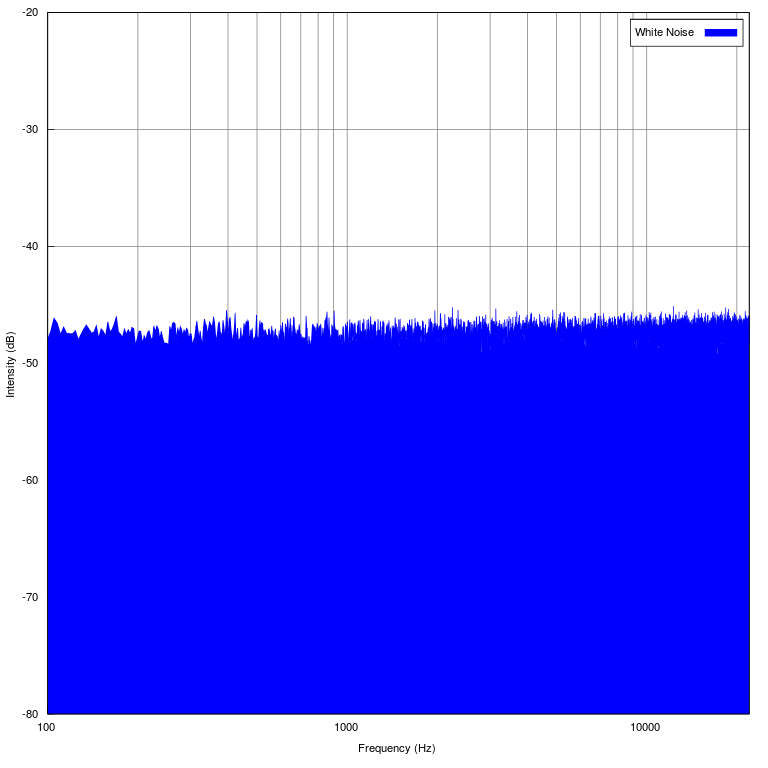
\includegraphics[width=0.45\textwidth]{WhiteNoise.png}
	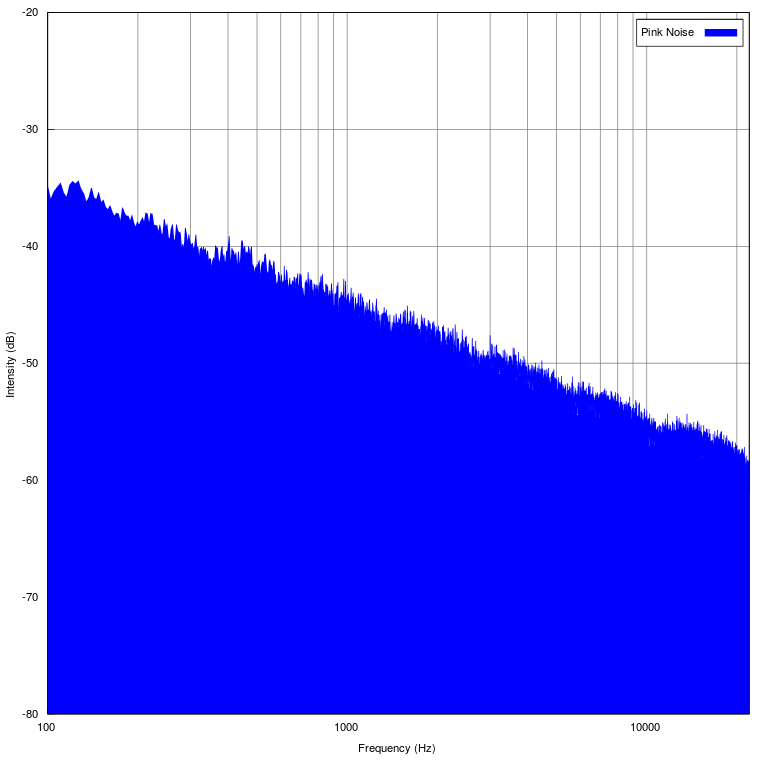
\includegraphics[width=0.45\textwidth]{PinkNoise.png}
\end{center}


\end{document}
